\section{问题四：波动电价下的扩展}
\subsection{价格预测与问题4-2}
未来实际价格不可见，故对电价同样采用式~\eqref{eq:forecast}的历史滚动预测，实际价格只用于事后结算。价格预测MAE和WAPE分别为0.0504元/kWh和6.66\%，预测与实际日均价格见图~\ref{fig:price}。
\begin{figure}[H]\centering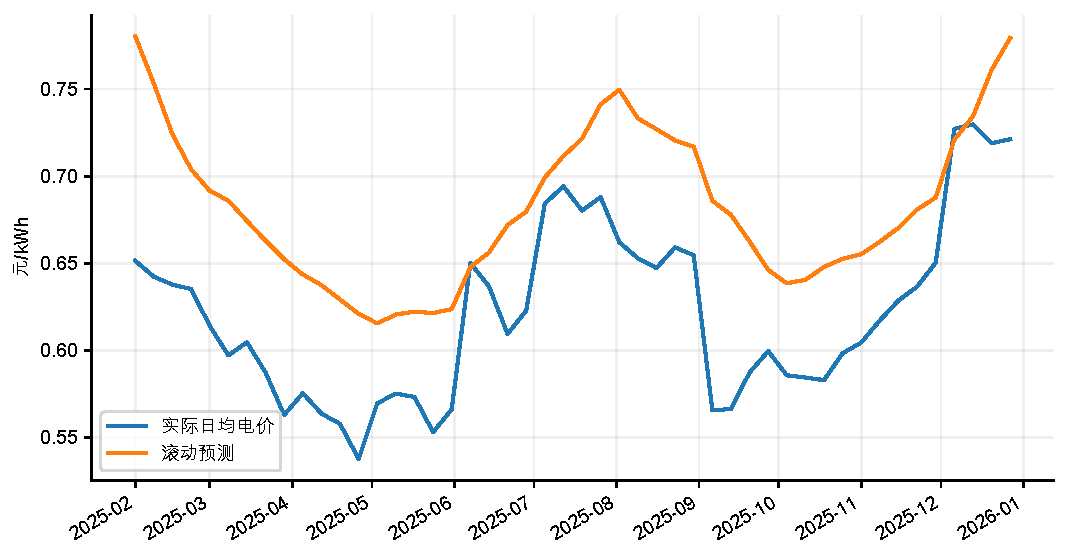
\includegraphics[width=0.90\textwidth]{../figures/fig06_price_forecast.pdf}
\caption{波动电价的历史滚动预测与实际值}\label{fig:price}\end{figure}
问题4-2将预测价格代入问题二的目标函数，实际价格结算后费用为16,163,346.40元；将问题二固定价策略直接用于波动价的基线为16,171,689.06元，前者降低8,342.66元，约0.05\%。改进幅度较小，表明当前简单价格预测对调度顺序的边际影响有限。
\subsection{问题4-3与综合比较}
问题4-3同时在发布时点更新光伏预测，并根据已观察价格偏差修正剩余时段的价格预测。滚动策略费用为16,977,176.53元，不调整基线为16,567,282.25元，滚动调整增加409,894.28元，说明当前结算规则下更新带来的收益仍不足以覆盖调整代价。
图~\ref{fig:compare}汇总四组主模型与基线。问题二和问题4-2改善费用，而问题三和问题4-3说明高调整罚金下全时点更新并非必然最优。
\begin{figure}[H]\centering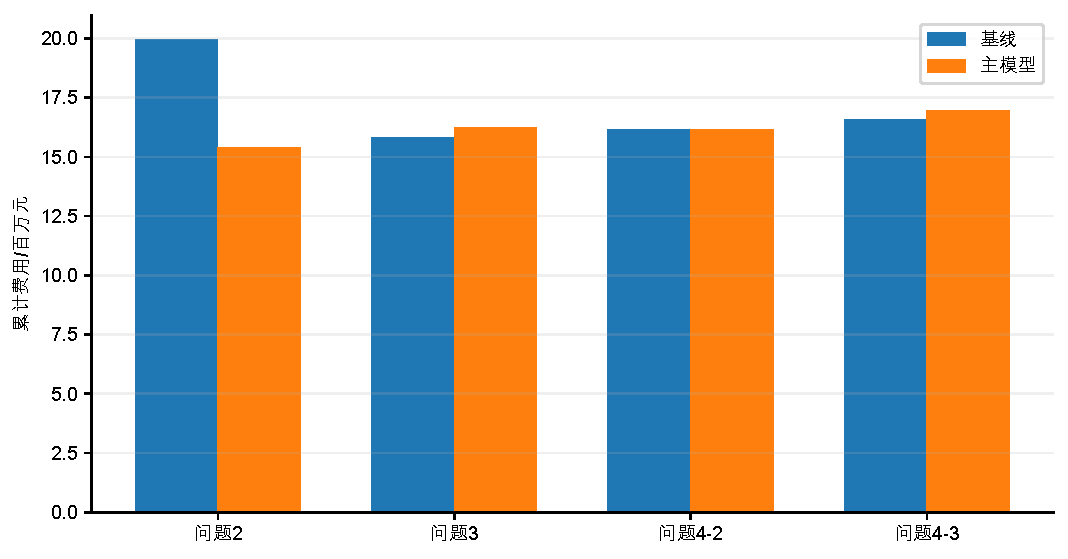
\includegraphics[width=0.92\textwidth]{../figures/fig03_model_comparison.pdf}
\caption{各问题主模型与对应基线累计费用比较}\label{fig:compare}\end{figure}
\begin{table}[H]\centering\caption{四个指定日期的主模型总费用（元）}\label{tab:selected}\small
\begin{tabular}{lrrrr}\toprule 日期 & 问题二 & 问题三 & 问题4-2 & 问题4-3\\\midrule
2025-03-20 & 45,655.77 & 57,498.21 & 46,925.61 & 59,045.90\\
2025-06-21 & 31,280.83 & 31,320.96 & 26,760.27 & 26,986.85\\
2025-09-23 & 56,667.56 & 51,011.60 & 59,231.53 & 53,384.07\\
2025-12-21 & 66,260.98 & 69,667.17 & 78,128.57 & 82,315.16\\\bottomrule
\end{tabular}\end{table}
